\section{Metodología de la investigación}

El presente trabajo se desarrolló mediante una metodología de investigación aplicada
con evaluación experimental. Dado que el problema abordado exigía intervenir un
simulador cuántico real, incorporar una estrategia de compresión sin pérdida de
precisión y verificar su efecto sobre memoria, tiempo y exactitud numérica, la
metodología se estructuró como un proceso de diseño, implementación y validación
comparativa. En consecuencia, el trabajo combinó revisión del estado del arte,
selección justificada de herramientas, diseño de una arquitectura de almacenamiento,
desarrollo de la solución e instrumentación experimental sobre cargas de trabajo
representativas.

\begin{figure}[H]
    \centering
    \caption{Metodología de investigación}
    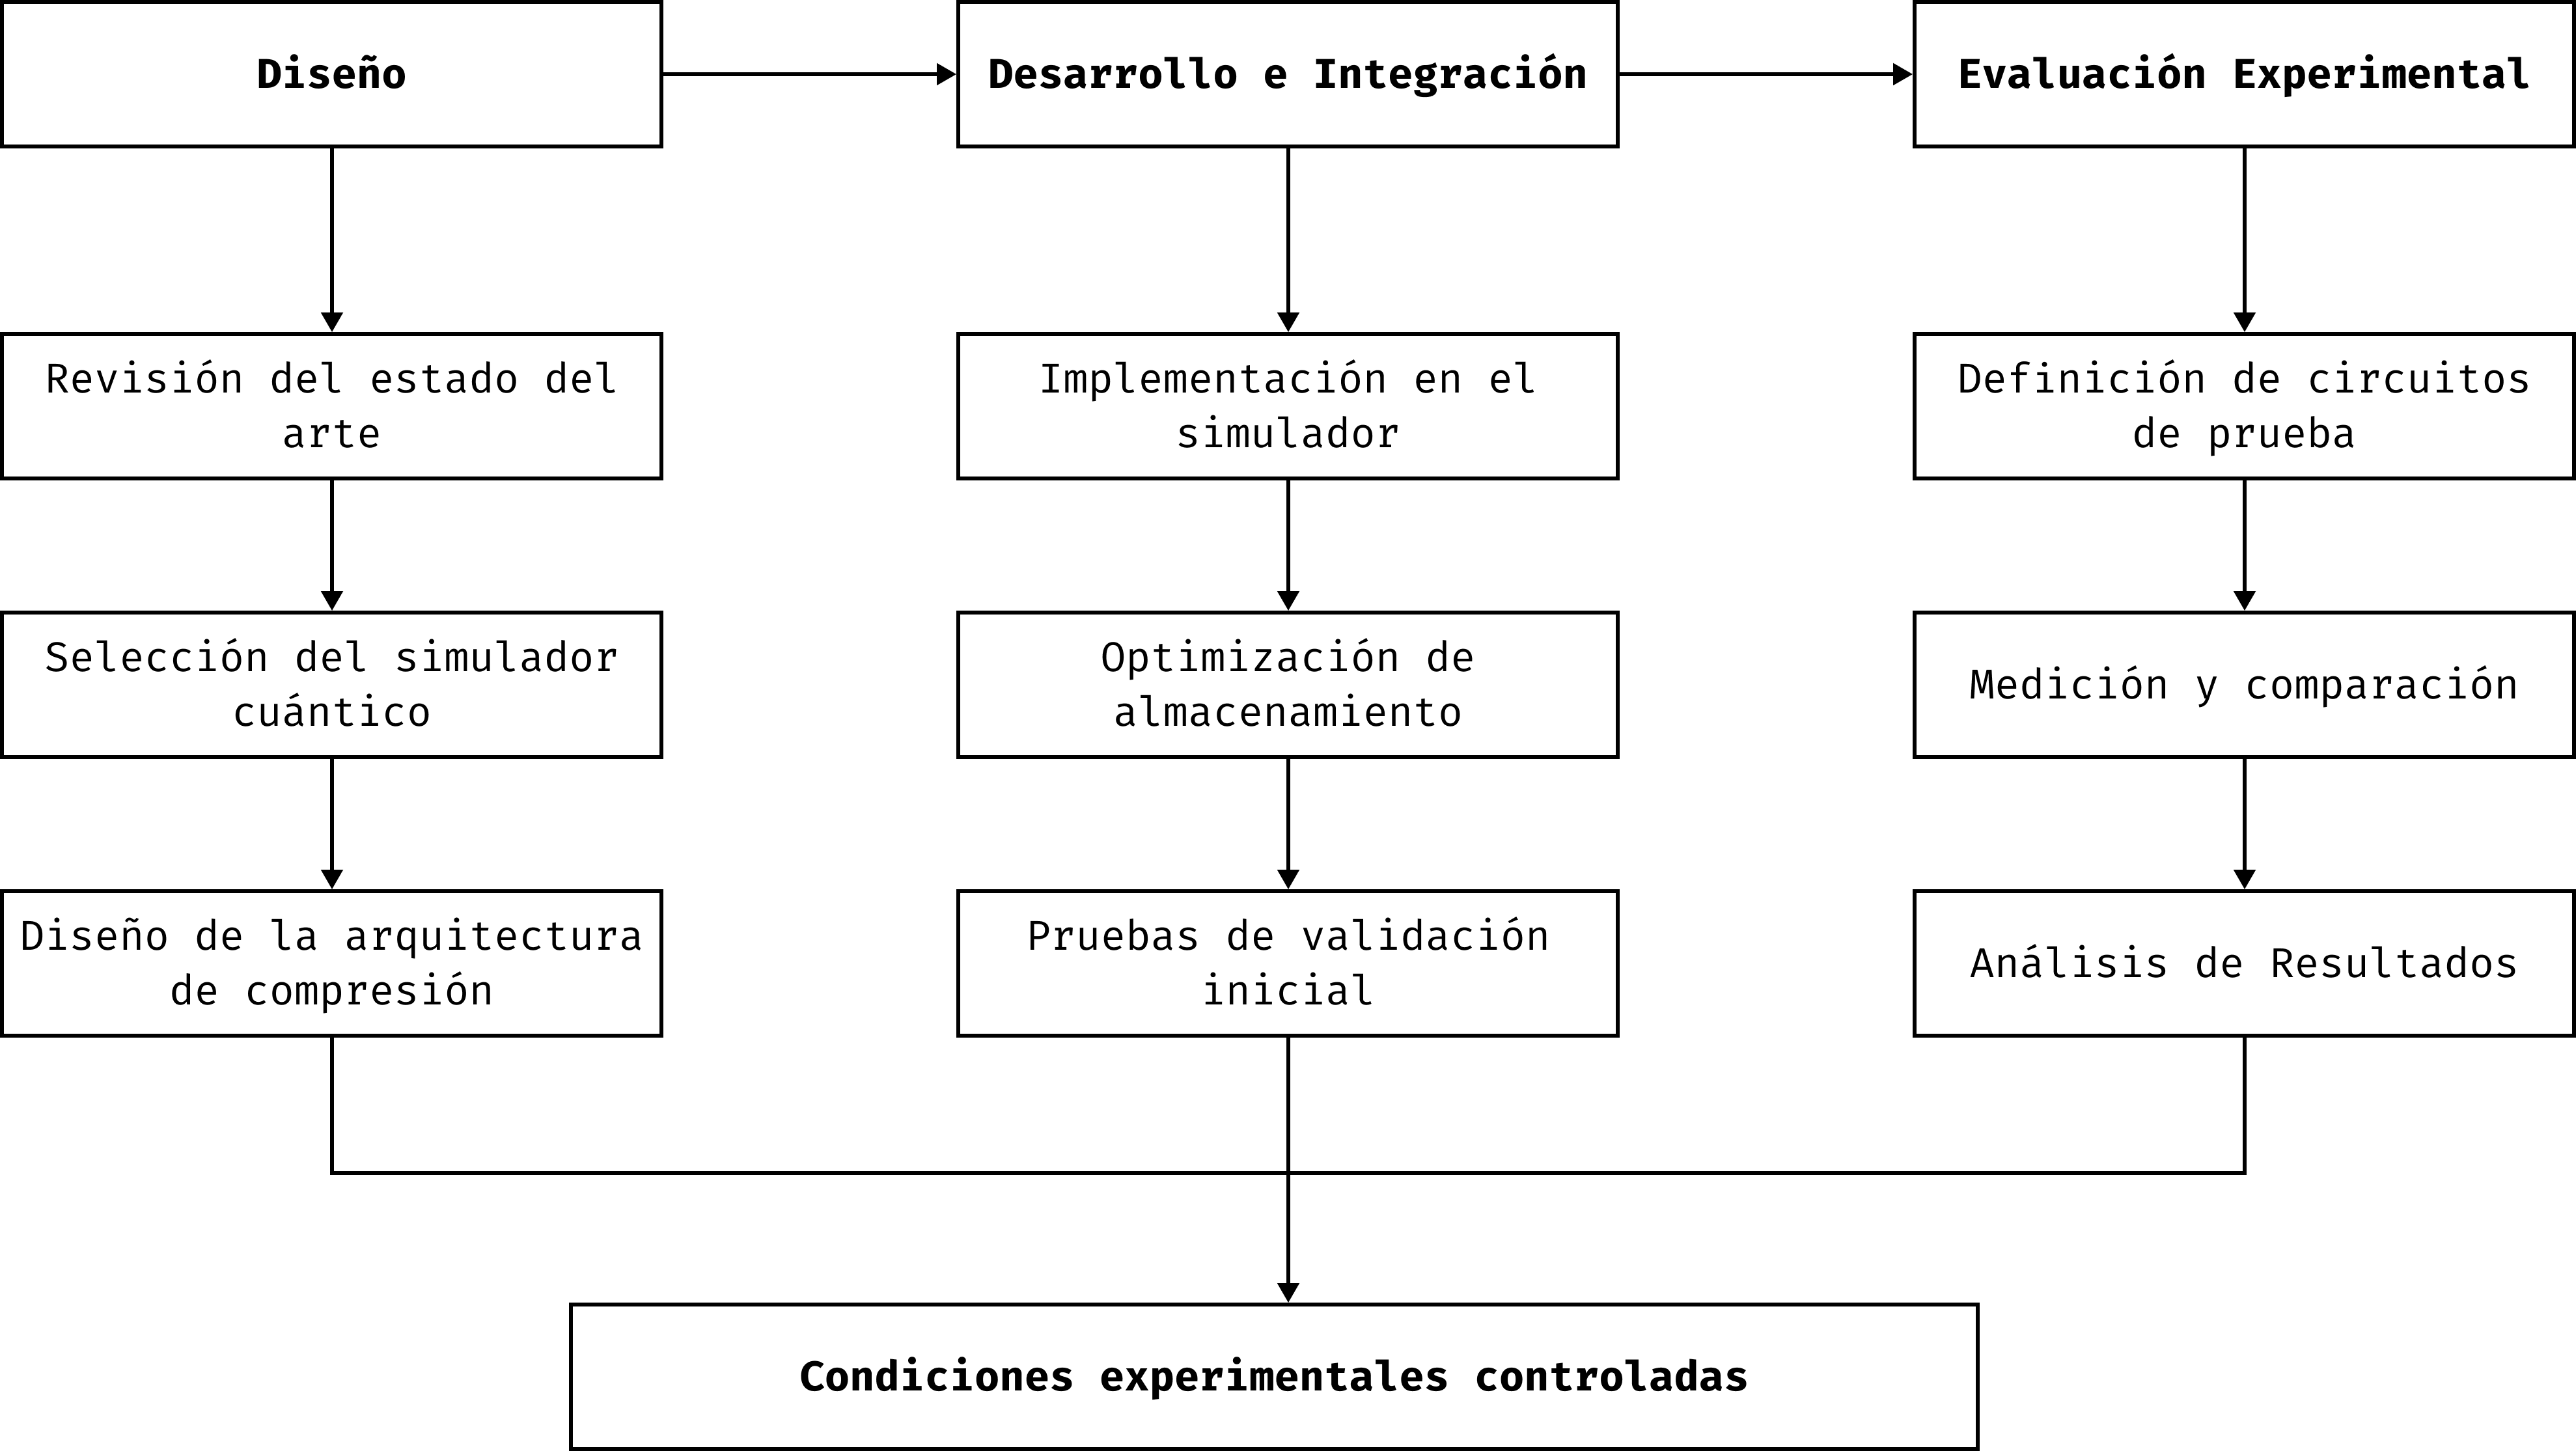
\includegraphics[width=1\linewidth]{images/metodologia.png}
    \label{fig:met}
\end{figure}

\subsection{\normalsize Diseño}

La fase de diseño estableció la base conceptual y técnica de la propuesta. En esta
etapa se realizó la revisión del estado del arte sobre simulación cuántica de estado
completo, compresión de datos de punto flotante y estrategias de optimización de
memoria, con énfasis en enfoques sin pérdida de precisión aplicables al vector de
estado. Esta revisión permitió identificar las alternativas existentes, sus limitaciones y
su pertinencia frente al problema específico de reducir la huella de memoria sin alterar
el resultado numérico de la simulación.

A partir de este análisis se definieron los criterios para la selección del simulador
cuántico base. Se consideraron aspectos como la apertura y modificabilidad del código
fuente, la facilidad de intervención sobre la representación del vector de estado, la
compatibilidad con optimizaciones de memoria, el soporte de paralelismo y la
posibilidad de instrumentar métricas experimentales. La selección se formalizó
mediante una matriz de evaluación ponderada entre las alternativas consideradas.

Finalmente, se definió la arquitectura general de la solución. En esta etapa se
establecieron la organización del vector de estado en bloques, los mecanismos de
compresión y descompresión selectiva, la estrategia de reutilización temporal de datos
y los puntos de integración con el simulador seleccionado. Con ello se delimitó el
marco de implementación de la propuesta y se fijaron los supuestos que orientarían su
evaluación posterior.

\subsection{\normalsize Implementación e integración de la estrategia}

La segunda fase correspondió al desarrollo de la estrategia diseñada y su integración en
el simulador seleccionado. El objetivo fue materializar la arquitectura propuesta en una
implementación funcional capaz de operar sobre el almacenamiento del vector de
estado sin modificar el modelo general de simulación.

Para ello se intervino el código fuente del simulador en los componentes asociados a la
representación, acceso y actualización del vector de amplitudes, incorporando el
esquema de almacenamiento comprimido sin pérdida. Esta integración incluyó la
gestión de bloques comprimidos, los procedimientos de recuperación y actualización de
datos, y los mecanismos requeridos para su persistencia durante la ejecución del
circuito.

De forma complementaria, se optimizó el esquema de acceso al almacenamiento con el
fin de controlar la sobrecarga asociada a la compresión y descompresión. Estas
adaptaciones buscaron favorecer la reutilización temporal de bloques y reducir accesos
innecesarios, de modo que el ahorro de memoria no implicara un deterioro desproporcionado
del tiempo de ejecución.

Una vez integrada la estrategia, se realizaron pruebas iniciales sobre circuitos de
validación para comprobar la estabilidad del desarrollo y verificar, en el caso de la
propuesta sin pérdida, la coincidencia exacta del estado final frente a la referencia no
comprimida.

\subsection{\normalsize Evaluación experimental}

La evaluación experimental se diseñó para determinar el efecto de la estrategia de
compresión sobre el comportamiento del simulador en términos de uso de memoria,
costo temporal y exactitud numérica. En particular, esta fase buscó establecer en qué
condiciones la compresión sin pérdida constituye una alternativa viable frente al
almacenamiento no comprimido y cómo se compara con una estrategia complementaria
de compresión con pérdida controlada.

La campaña experimental se planteó sobre cargas de trabajo con comportamientos de
compresibilidad contrastantes. Para ello se seleccionaron dos familias de circuitos: la
Transformada Cuántica de Fourier (QFT) y el algoritmo de búsqueda de Grover. Esta
selección permitió evaluar la propuesta en escenarios con estructuras de estado y
patrones de acceso diferentes, evitando que la valoración dependiera de un único tipo
de circuito.

La comparación se realizó entre tres escenarios: una ejecución de referencia sin
compresión, una ejecución con la estrategia de compresión sin pérdida integrada en el
simulador y una ejecución con una estrategia de compresión con pérdida controlada.
Bajo esta organización fue posible analizar tanto el ahorro de memoria como la
sobrecarga temporal y el comportamiento de la exactitud numérica en cada enfoque.

Las métricas principales de evaluación fueron el tiempo total de ejecución y el uso
máximo de memoria durante la simulación. Adicionalmente, la exactitud se evaluó de
forma diferenciada según la naturaleza de la estrategia comparada. En la propuesta sin
pérdida, el criterio de validación consistió en verificar igualdad exacta entre el estado
final comprimido y la referencia no comprimida:

\[
\alpha_i^{(\text{ref})} = \alpha_i^{(\text{comp})} \quad \forall i.
\]

En la estrategia con pérdida controlada, la discrepancia respecto a la referencia se
resumió mediante el error absoluto máximo:

\[
e_{\text{abs}} = \max_i \left|\alpha_i^{(\text{ref})} - \alpha_i^{(\text{comp})}\right|.
\]

Con el fin de reducir la dependencia de configuraciones particulares, en Grover se
consideraron múltiples instancias por tamaño, mientras que en QFT se evaluó una
instancia por familia de entrada y por número de qubits. Finalmente, la exactitud se
verificó mediante la exportación y comparación completa del vector de amplitudes
frente a la referencia no comprimida. En la estrategia sin pérdida, esta comparación
permitió confirmar igualdad exacta amplitud por amplitud; en la estrategia con pérdida,
el mismo procedimiento se empleó para calcular el máximo error absoluto. De este
modo, la evaluación experimental quedó orientada a establecer los compromisos entre
memoria, tiempo y exactitud en las estrategias de almacenamiento consideradas.